% ============================================================
% C3 — Adaptive re-fan-out: method (Sec. 4.4) + results (Sec. 5.4)
%       + appendix (loop details) + pending-experiment placeholders
% Paste-ready for the EACL/ACL Overleaf template.
% Requires: \usepackage{booktabs} \usepackage{graphicx}
% Figures: reports/paper/figures/*.pdf — regenerate with
%   .venv/bin/python scripts/make_paper_figures.py
% Cross-refs assumed elsewhere in the paper:
%   \label{sec:benchmark}            (benchmark / leak-free judging section)
%   \label{sec:results-placement}    (C1 placement results subsection)
% Every number is traceable to a repo artifact noted in a % comment.
% PLACEHOLDER protocol: blocks marked  %% PENDING(<what>)  are commented out
% until the corresponding runs exist (Llama replication, hand-off checks).
% ============================================================

% ============================================================
% Sec. 4.4 — method (paste inside the agent/system section)
% ============================================================
\subsection{Adaptive Re-Fan-Out}
\label{sec:method-refanout}

Static fan-out commits to one round of retrieval regardless of what comes
back. Our \emph{adaptive re-fan-out} loop instead retries the whole fan-out
until an in-loop judge deems the evidence sufficient. Each round (i)~generates
$k{=}4$ persona-conditioned queries --- round~1 from scratch, later rounds
from the judge's feedback; (ii)~executes them; and (iii)~has an LLM
\emph{retrieval judge} score the retrieved evidence for coverage on an
anchored 1--5 scale and list what is still missing. The judge is sampled
three times and averaged to suppress single-call noise, and it is
threshold-blind: a separate controller approves the round when its score
reaches a threshold $\tau$, synthesizing the answer from that round's
evidence alone, and otherwise discards the round and retries (up to six
rounds; on exhaustion, the best-scoring round is used). The judge sees only
agent-visible inputs --- never the evaluation rubric or the latent profile
(\S\ref{sec:benchmark}). Full loop details are in
Appendix~\ref{app:refanout-details}.
% mechanism: adaptive_refanout.py; leak-free contract: no rubrics import

\paragraph{Judge calibration.}
With naive score anchors the judge rated 10 of 12 first fan-outs a 4 or 5,
so the loop almost never engaged. We tightened the anchors (a top score
additionally requires corroboration and explicit caveat coverage, and the
judge defaults to the lower band when unsure), which spreads first-round
scores and makes $\tau\in\{3,4,5\}$ three distinct operating points, from
loop-off ($\tau{=}3$) to full persistence ($\tau{=}5$)
(Figure~\ref{fig:recalibration}, Appendix~\ref{app:refanout-details}). The
anchors were frozen on a 12-pair smoke set before the main grid ran, and no
rubric-aware evaluation judge was ever tuned.
% refanout_judge_recalibration.md (verified before/after)

\paragraph{One run, every $\tau$.}
Because the judge is threshold-blind and revisions depend only on its
threshold-blind feedback, a run's per-round trajectory is independent of
$\tau$: the threshold only decides where the loop stops reading it. We
therefore run each pair once at full persistence, logging every round's
evidence, and derive each smaller $\tau$'s outcome post hoc by re-synthesizing
from its stop round. The $\tau$ conditions thus differ only in stopping
behavior, never in sampled trajectories.
% derive_tau_grid.py docstring ("t5 is a superset" argument)

% ============================================================
% Sec. 5.4 — results (paste inside the Experiments section)
% ============================================================
\subsection{Does Adaptive Re-Fan-Out Help?}
\label{sec:results-refanout}

We run the loop on all 72 query--persona pairs with $k{=}4$ queries per round,
a six-round cap, and $\tau\in\{3,4,5\}$, using the hardened synthesizer (an
intent-inferring, grounding-guarded synthesis prompt) as the default final
query; all conditions share generation trajectories by construction
(\S\ref{sec:method-refanout}).
% setup: adaptive_refanout_v1, gemini-3.5-flash, seed 42; runs_v2synth_grid.jsonl
The threshold genuinely changes loop behavior: the mean stop round rises from
1.08 ($\tau{=}3$) to 1.54 ($\tau{=}4$) to 4.50 ($\tau{=}5$), and at
$\tau{=}5$ the loop re-fans for 55 of 72 pairs --- the sweep exercises
adaptive behavior rather than degenerating to a single fan-out.
% mean stop rounds computed from runs_v2synth_grid.jsonl (num_refanout_rounds)

\begin{figure*}[t]
\centering
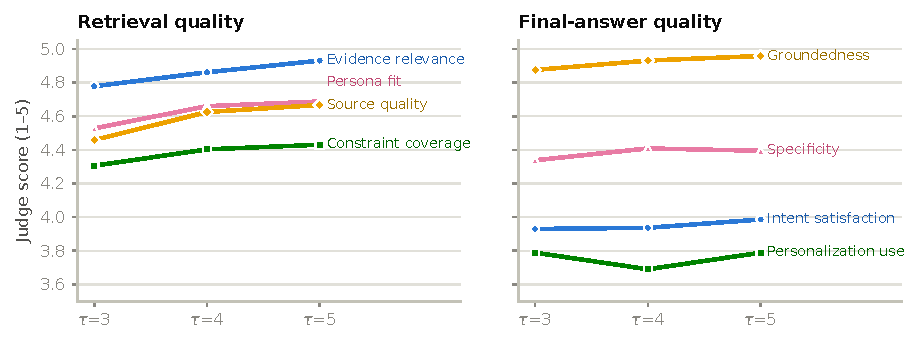
\includegraphics[width=\textwidth]{figures/refanout_decoupling.pdf}
\caption{Adaptive re-fan-out under increasing persistence ($\tau{=}3$: loop
off; $\tau{=}5$: full persistence; 72 pairs, hardened synthesizer). Retrieval
quality (left) climbs monotonically with $\tau$, while final-answer quality
(right, same scale) stays flat --- the loop improves the evidence, not the
answer.}
% data: outputs/adaptive_refanout_v1/synth_tau_frontier.csv (v2 rows)
%% PENDING(llama): swap in figures/refanout_decoupling_llama.pdf as a second
%% row of this figure* (or a stacked variant) once the Llama replication runs.
\label{fig:refanout-decoupling}
\end{figure*}

\begin{table}[t]
\centering
\small
\begin{tabular}{lcccc}
\toprule
 & $\tau{=}3$ & $\tau{=}4$ & $\tau{=}5$ & $\Delta_{3\to5}$ \\
\midrule
\multicolumn{5}{l}{\textit{Retrieval quality}} \\
Evidence relevance   & 4.78 & 4.86 & 4.93 & $+0.15$ \\
Constraint coverage  & 4.31 & 4.40 & 4.43 & $+0.13$ \\
Persona fit          & 4.53 & 4.66 & 4.69 & $+0.16$ \\
Source quality       & 4.46 & 4.63 & 4.67 & $+0.21^{*}$ \\
\midrule
\multicolumn{5}{l}{\textit{Final-answer quality}} \\
Intent satisfaction  & 3.93 & 3.94 & 3.99 & $+0.06$ \\
Personalization use  & 3.79 & 3.69 & 3.79 & $\phantom{+}0.00$ \\
Specificity          & 4.34 & 4.41 & 4.39 & $+0.06$ \\
Groundedness         & 4.88 & 4.93 & 4.96 & $+0.08$ \\
\bottomrule
\end{tabular}
\caption{Judge scores by loop persistence $\tau$ (72 pairs, hardened
synthesizer). Retrieval quality climbs while final-answer quality is
statistically flat ($^{*}$: bootstrap 95\% CI excludes zero; intent
$\Delta_{3\to5}=+0.06$, CI $[-0.10,+0.21]$).}
% means: synth_tau_frontier.csv (v2 rows); intent CI: refanout_tau_analysis.ipynb
% TODO(colleague): pull remaining Delta_{3->5} CIs from v2synth_tau_gains.csv
% (t3_to_t5 rows) and add stars accordingly.
\label{tab:refanout-tau}
\end{table}

%% PENDING(llama): model-sweep version of Table~\ref{tab:refanout-tau}.
%% Uncomment and fill the Llama column when the replication lands; keep the
%% same row order so the two tables diff cleanly.
% \begin{table}[t]
% \centering\small
% \begin{tabular}{lcc}
% \toprule
%  & Gemini-3.5-Flash & Llama-3.3-70B \\
% \midrule
% Retrieval source quality $\Delta_{3\to5}$ & $+0.21^{*}$ & --- \\
% Retrieval constraint coverage $\Delta_{3\to5}$ & $+0.13$ & --- \\
% Intent satisfaction $\Delta_{3\to5}$ & $+0.06$ & --- \\
% Synthesis lift (base$\to$hardened, intent) & $+0.72^{*}$ & --- \\
% \bottomrule
% \end{tabular}
% \caption{Cross-model replication of the re-fan-out findings. PENDING: Llama
% runs (identical grid, prompts, and judges; only the agent backbone swaps).}
% \label{tab:refanout-models}
% \end{table}

\begin{figure}[t]
\centering
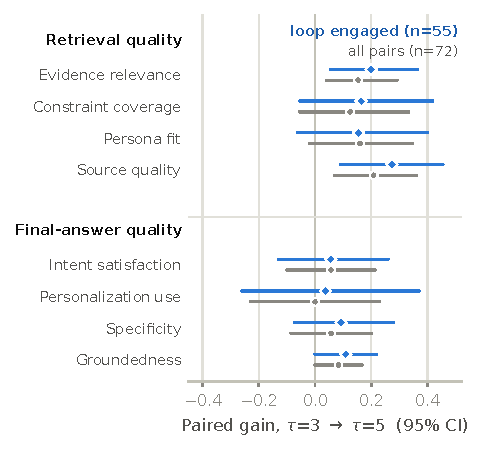
\includegraphics[width=\columnwidth]{figures/tau_gains_forest.pdf}
\caption{Paired per-pair gains from turning the loop on
($\tau{=}3\to\tau{=}5$) with bootstrap 95\% CIs, on all 72 pairs and on the
55 pairs whose loop actually re-fanned. Every retrieval gain sits right of
zero --- larger on the engaged subset --- while every final-answer gain
straddles it. Engagement is determined by the first round's judge score,
which is identical across $\tau$ arms, so the subset is fixed pre-treatment.}
% data: v2synth_tau_gains.csv + engaged_v2_tau_gains.csv (t3_to_t5 rows)
%% PENDING(llama): figures/tau_gains_forest_llama.pdf companion.
\label{fig:tau-gains-forest}
\end{figure}

\paragraph{Re-fan-out improves what it optimizes: retrieval.}
Figure~\ref{fig:tau-gains-forest} shows the paired gains from turning the
loop on: on the full set, source quality improves $+0.21$
(CI $[0.07, 0.36]$) and evidence relevance $+0.15$ (CI $[0.04, 0.29]$), and
the gains grow where the loop actually engages --- on the 55 re-fanned pairs,
source quality reaches $+0.27$ (CI $[0.09, 0.46]$) and evidence relevance
$+0.20$ (CI $[0.05, 0.36]$). Absolute levels
(Figure~\ref{fig:refanout-decoupling}, left; Table~\ref{tab:refanout-tau})
rise monotonically with $\tau$ even though first fan-outs already score high,
so the headroom is small. The loop does exactly what its in-loop judge asks
of it: later rounds retrieve better-sourced, better-targeted evidence. With
${\sim}18$ metrics tracked, isolated significance stars deserve caution; we
rest this claim on the pattern instead --- the retrieval gains are monotone
in $\tau$, consistent across the full and engaged sets, and largest where
first-round coverage was weakest.

\paragraph{The retrieval gains do not reach the answer.}
Intent satisfaction moves $+0.06$ (CI $[-0.10,+0.21]$) across the same sweep,
and every answer-side CI in Figure~\ref{fig:tau-gains-forest} straddles zero.
Read as an equivalence bound, the sweep rules out intent gains larger than
${\approx}0.21$ --- under a third of the placement effects in
\S\ref{sec:results-placement} and, as shown next, under a third of what the
synthesis prompt delivers on the same evidence. The decoupling is not an
artifact of pairs whose first fan-out was already approved: on the engaged
subset the retrieval gains \emph{grow} while intent stays at $+0.06$ (n.s.).
% engaged subset: engaged_v2_tau_gains.csv / refanout_tau_analysis.ipynb
A pre-specified stratification by first-round coverage --- a predictor judged
before the loop re-fans, not the realized outcome --- reinforces the picture:
in the weakest band (first-round coverage $\le 3$, $n{=}14$), where the loop
works hardest and its retrieval gain is largest ($+0.36$ source quality), we
find no positive answer effect (intent $-0.21$, CI $[-0.43, 0.00]$; a small
stratum, so we read this as an absence of gain, not a reliable loss).
% lowcov_cut.csv; framing per refanout_tau_analysis.ipynb

\begin{figure}[t]
\centering
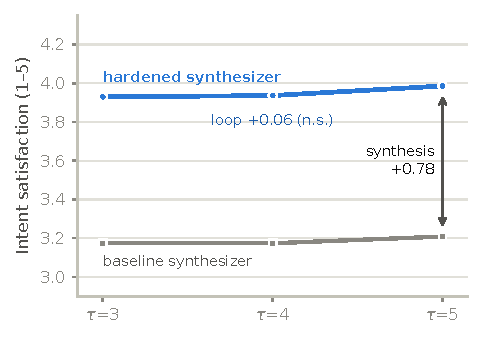
\includegraphics[width=\columnwidth]{figures/synthesis_vs_loop.pdf}
\caption{Where answer quality is won. Swapping the synthesis prompt lifts
intent satisfaction by $+0.74$--$+0.79$ at every persistence level (plotted:
per-$\tau$ means; gap $0.78$ at $\tau{=}5$), while pushing the loop from off
($\tau{=}3$) to full persistence ($\tau{=}5$) moves it $+0.06$ (n.s.) ---
even the loop's CI ceiling ($+0.21$) is under a third of the synthesis
lift.}
% data: synth_tau_frontier.csv (baseline + v2 rows)
%% PENDING(llama): figures/synthesis_vs_loop_llama.pdf companion.
\label{fig:synthesis-vs-loop}
\end{figure}

\paragraph{Answer quality is a synthesis lever, not a loop lever.}
Holding evidence fixed at every $\tau$ and swapping only the final synthesis
prompt isolates where answer quality is won
(Figure~\ref{fig:synthesis-vs-loop}). The hardened prompt --- which
explicitly infers the user's latent intent, applies persona constraints, and
enforces a grounding guard --- lifts intent satisfaction by $+0.74$ to
$+0.79$ at every persistence level (paired on the derived grid; $+0.79$,
CI $[0.59, 1.00]$ at $\tau{=}5$), with a small \emph{improvement} in
groundedness ($+0.07$) and fewer unsupported claims. An independent live
re-execution of the $\tau{=}5$ arm with both prompts reproduces the lift
($+0.72$, CI $[0.54, 0.90]$).
% derived grid: synth_improve_by_tau.csv; live replication: synth_ablation_summary.csv (d_v2_base)
An intermediate prompt without the grounding guard bought more intent
($+1.06$) but paid for it in faithfulness (groundedness $-0.29$, unsupported
claims $+0.31$), which the final prompt repairs.
% synth_ablation_summary.csv, d_v1_base and d_v2_v1 rows
The attribution is stark even at the loop's most favorable reading: the
synthesis effect ($+0.79$) is ${\sim}3.8\times$ the \emph{upper edge} of the
loop's CI ($+0.21$), and ${\sim}13\times$ its point estimate; the
synthesis--loop interaction is negligible.

\paragraph{An answer-judging loop shows the same pattern (pilot).}
A natural objection is that the loop optimizes the wrong objective: its judge
asks ``what evidence is missing?'', which is only loosely related to answer
quality. We therefore piloted a variant that synthesizes a draft answer every
round and re-fans on a leak-free \emph{answer critic}'s reported gaps
(20 pairs). By the critic's own measure re-fanning improves drafts ($+0.77$),
yet rubric-scored intent shows no sign of moving ($+0.05$ overall; $0.00$ on
the 11 pairs where the loop changed the answer --- pilot-scale, so
corroborative rather than confirmatory).
% answer_critic_loop_pilot.md (pilot tables)
The variant's genuine value is diagnostic: it flags 39\% of rounds as
synthesis-bound rather than retrieval-bound and catches fabricated statistics
--- a faithfulness and observability tool rather than an answer-quality
mechanism.

\paragraph{Takeaway.}
Adaptive re-fan-out earns its keep on retrieval quality and on observability;
final-answer quality on this benchmark is won at synthesis. The two levers
are near-orthogonal, so practitioners should spend loop budget when evidence
quality is the product surface, and invest in persona-conditioned synthesis
when answer quality is.

%% PENDING(hand-off): robustness paragraph. Uncomment once the two
%% scoring-only checks exist:
%%   (1) cross-seed check on final metrics — score runs_k3judge_rep2.jsonl
%%       (seed 123) with the final-answer judges vs. the seed-42 twin;
%%   (2) evaluator repeatability — double-score a subset with the same judge.
% \paragraph{Robustness.}
% Final-answer scores are stable across pipeline seeds (12-pair replicate,
% seeds 42 vs.\ 123: mean per-pair difference XX, max XX) and across repeated
% judging of identical answers (evaluator repeatability $\sigma$ = XX);
% differences below ${\sim}$XX should be read as noise.

% ============================================================
% Appendix — paste after \appendix
% ============================================================
\section{Adaptive Re-Fan-Out: Loop Details}
\label{app:refanout-details}

\paragraph{In-loop judge denoising.}
Single judge calls exhibit heavy-tailed noise (isolated $\pm2$ swings on the
1--5 scale; pooled within-call $\sigma\approx0.36$). Sampling the judge three
times per round and averaging reduces this to $\sigma\approx0.21$ and yields
fractional coverage scores, giving $\tau$ a finer sweep than integer scores
allow. The union of the samples' missing-evidence lists and the most critical
sample's feedback seed the next round's fan-out, with an explicit instruction
to change search direction rather than rephrase.
% c3_refanout_pipeline_hardening.md (noise investigation)

\paragraph{Best-round fallback.}
Revised fan-outs can drift: a retried round sometimes scores below its
predecessor. On exhausting the round cap the loop therefore synthesizes from
the highest-coverage round rather than the last one. Every round's evidence
is logged, which is also what makes the round cap a nested, post-hoc variable.

\paragraph{Judge recalibration.}
With naive anchors, 10 of 12 smoke-set first fan-outs scored 4--5 (mean 1.17
rounds; the loop retried twice). The recalibrated anchors require, for a top
score, that evidence cover the core ask \emph{and} the user-relevant
constraints \emph{and} corroborate across sources \emph{and} (for
consequential topics) include explicit caveats; the judge is instructed to
default to the lower band when unsure and to score relative to what a strong
answer for \emph{this} user requires. On the same 12 pairs the round-1 score
histogram spreads from $\{1{:}1, 3{:}1, 4{:}4, 5{:}6\}$ to
$\{3{:}5, 4{:}4, 5{:}3\}$ (Figure~\ref{fig:recalibration}); mean rounds rise
from 1.17 to 1.50, and the loop retries on 5 of 12 pairs, 4 of which improve
their coverage. At $\tau{=}5$ the loop averages 2.08 rounds with 6 of 12
pairs reaching the round cap, confirming that the cap binds only at high
persistence.
% refanout_judge_recalibration.md; runs_tau5_smoke.jsonl

\begin{figure}[t]
\centering
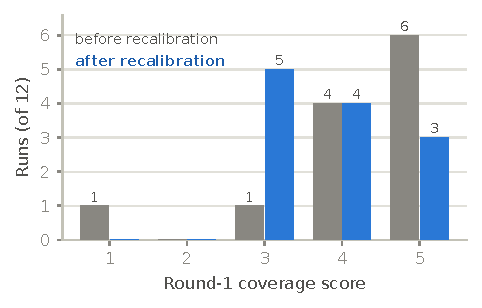
\includegraphics[width=\columnwidth]{figures/judge_recalibration.pdf}
\caption{Round-1 coverage scores on the same 12-pair smoke set before and
after recalibrating the retrieval judge's anchors. The compressed top band
(before) made every $\tau$ approve immediately; the recalibrated spread makes
$\tau\in\{3,4,5\}$ distinct operating points.}
% data recomputed from outputs/adaptive_refanout_v1/runs.jsonl (before) and
% runs_recalibrated_smoke.jsonl (after) by scripts/make_paper_figures.py
\label{fig:recalibration}
\end{figure}

\paragraph{Hyperparameters and scope.}
$k{=}4$ queries per round; round cap 6; judge samples $K{=}3$; single seed
(42); planner, synthesizer, and judges all use the same backbone
(gemini-3.5-flash). We did not sweep $k$ or the round cap, and retrieval cost
is out of scope (quality only).
%% PENDING(hand-off): add the cross-seed and evaluator-repeatability numbers
%% here once scored (see Sec.~\ref{sec:results-refanout} robustness stub);
%% cite both in Limitations alongside the shared-backbone caveat.
